\documentclass{article}
%Nu tester jeg lige igen
% Language setting
% Replace `english' with e.g. `spanish' to change the document language
\usepackage[danish]{babel}
% Set page size and margins
% Replace `letterpaper' with `a4paper' for UK/EU standard size
\usepackage[a4paper,top=2cm,bottom=2cm,left=3cm,right=3cm,marginparwidth=1.75cm]{geometry}

% Useful packages
\usepackage{amsmath}
\usepackage{graphicx}
\usepackage[colorlinks=true, allcolors=blue]{hyperref}
\usepackage{array}

\title{CDIO delopgave 1}
\author{Jakob Agergaard}


\begin{document}




\begin{titlepage}
\begin{center}

    
\includegraphics[width=0.25\textwidth]{Billeder/DTULogo.png} \\
    \vspace{0.5cm}
    \Large
    \textbf{02314\hspace{1cm}62531\hspace{1cm}62532} \\
    Indledende programmering, Udviklingsmetoder til IT-systemer og Versionsstyring og testmetoder
    \vspace{0.4cm}
    \hrule
    
    \vspace*{0.5cm}
    \huge
    \textbf{CDIO delopgave 1}\\
    \LARGE
    Gruppe 17
    \vspace{0.5cm}
    \hrule
    \vspace{0.2cm}

    \large
    \begin{tabular}{m{10em} m{8em} m{8em} m{10em}}
    Jakob Skov Agergaard\vfill s224570 & 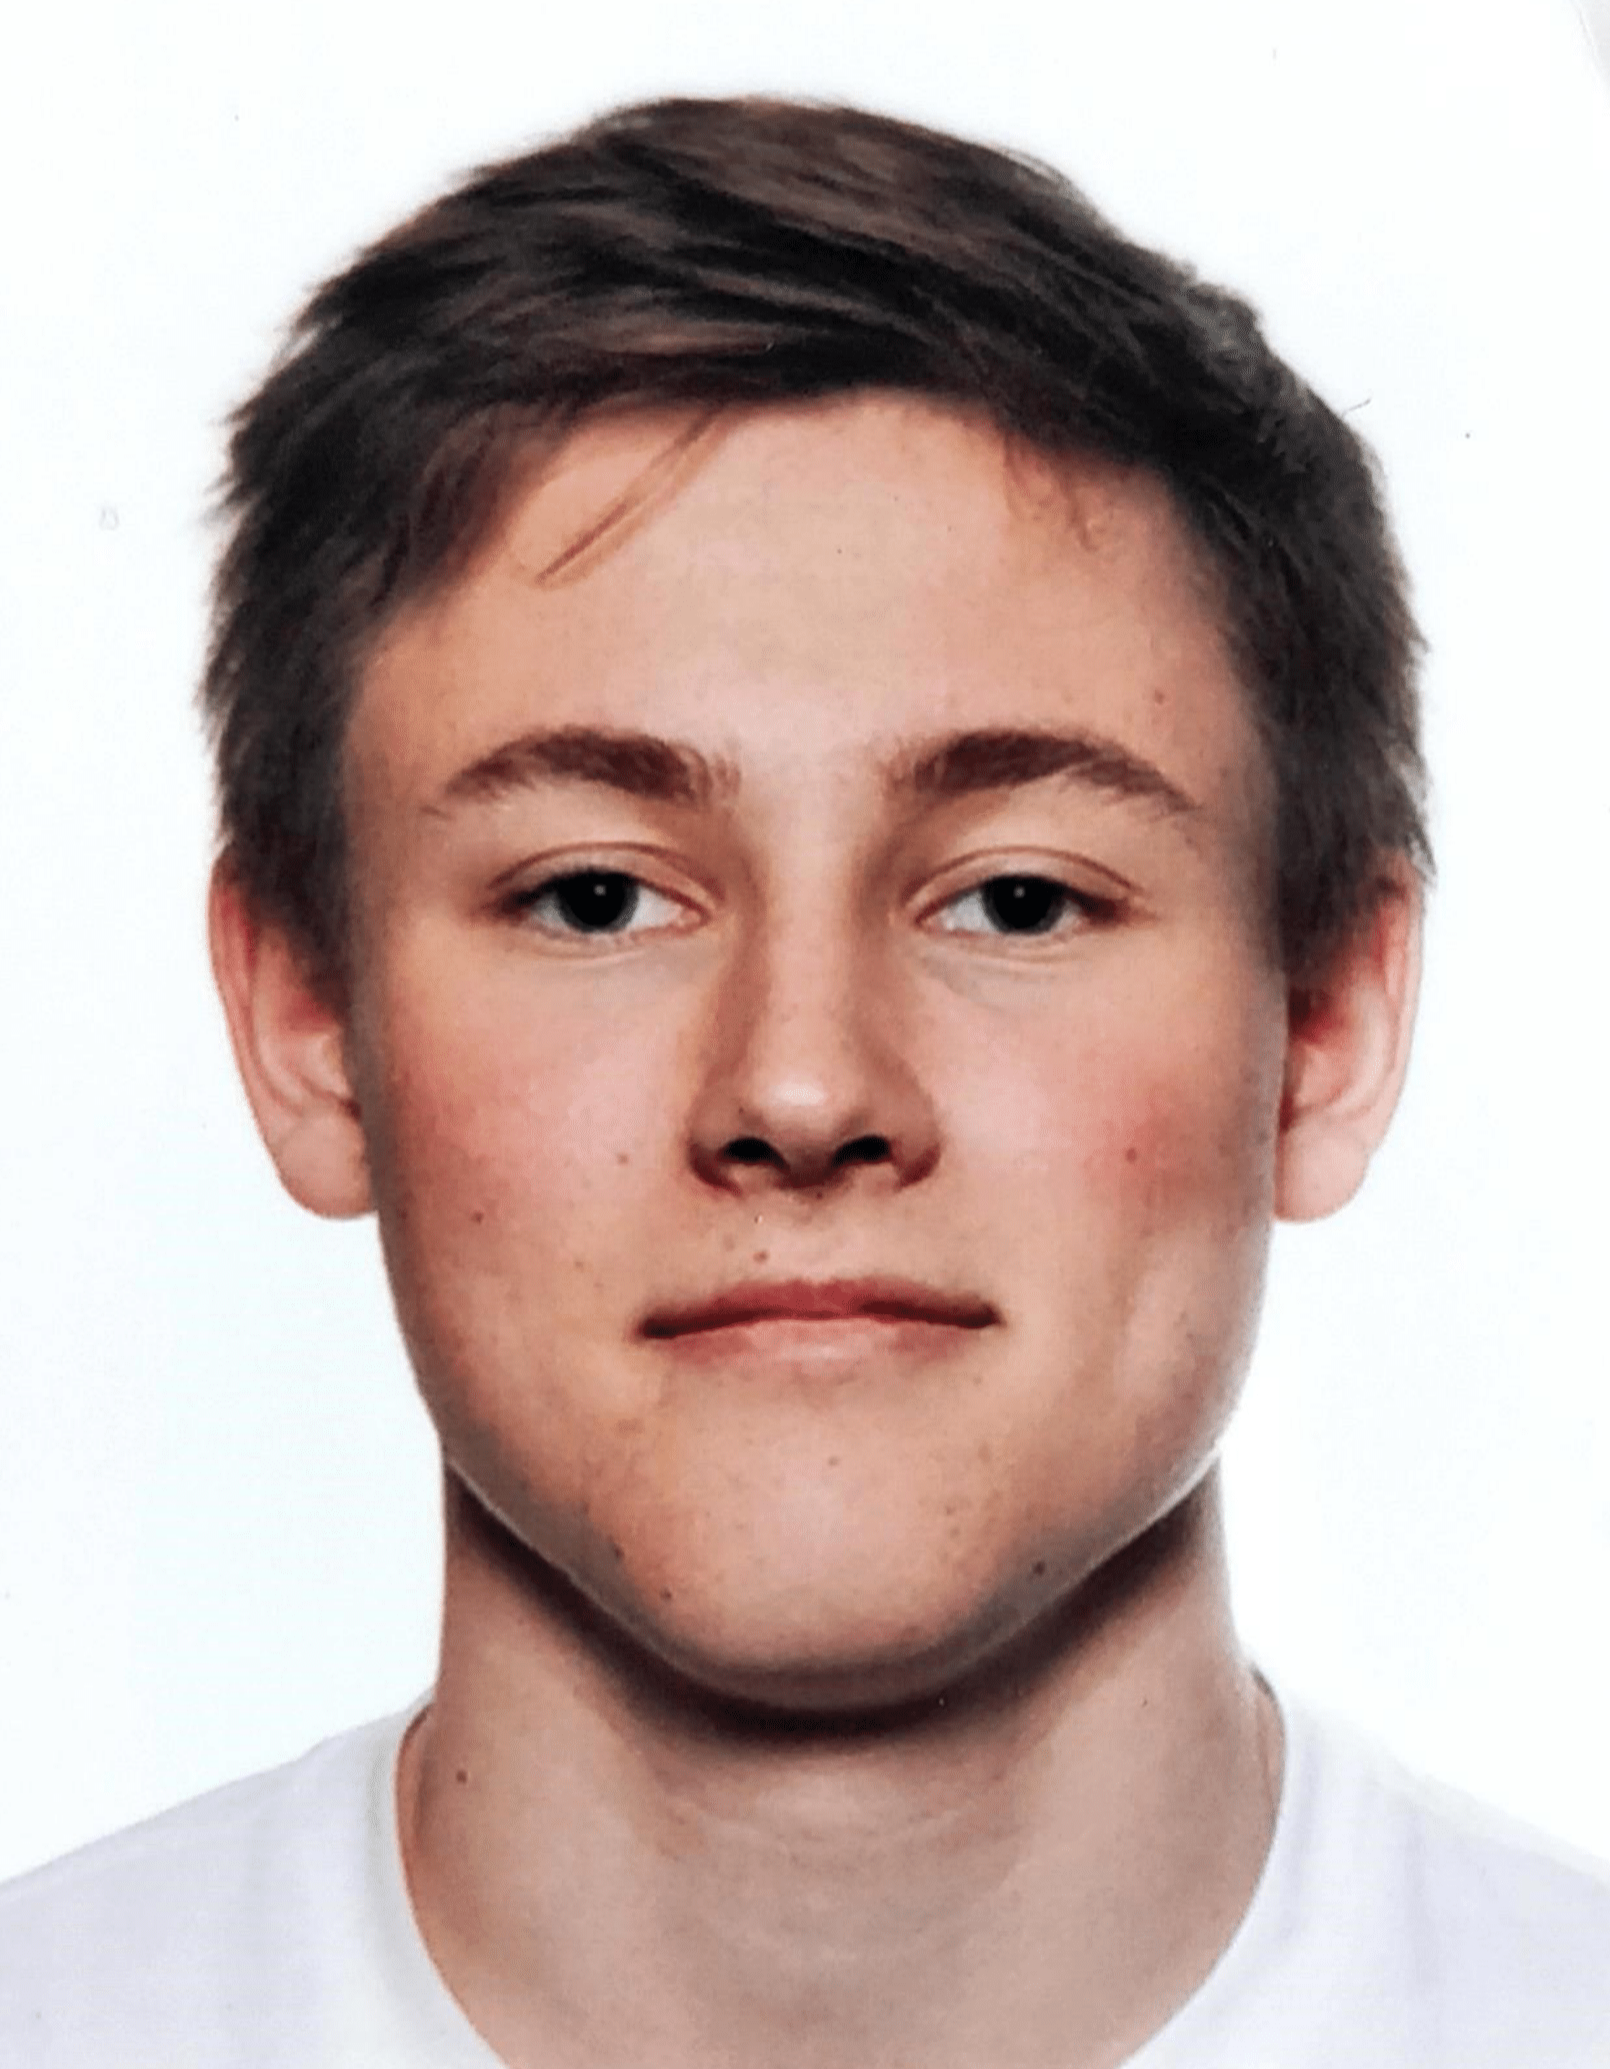
\includegraphics[width=0.2\textwidth]{Billeder/JakobFoto.png} & 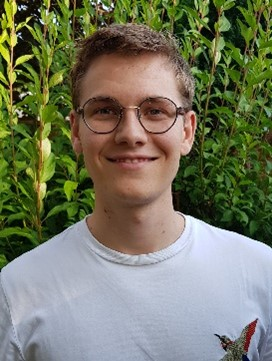
\includegraphics[width=0.2\textwidth]{Billeder/PhilipFoto.jpg} & Philip Muff Førrisdahl\vfill s224566 \\
    Mads Fogelberg Hansen\vfill s224563 & 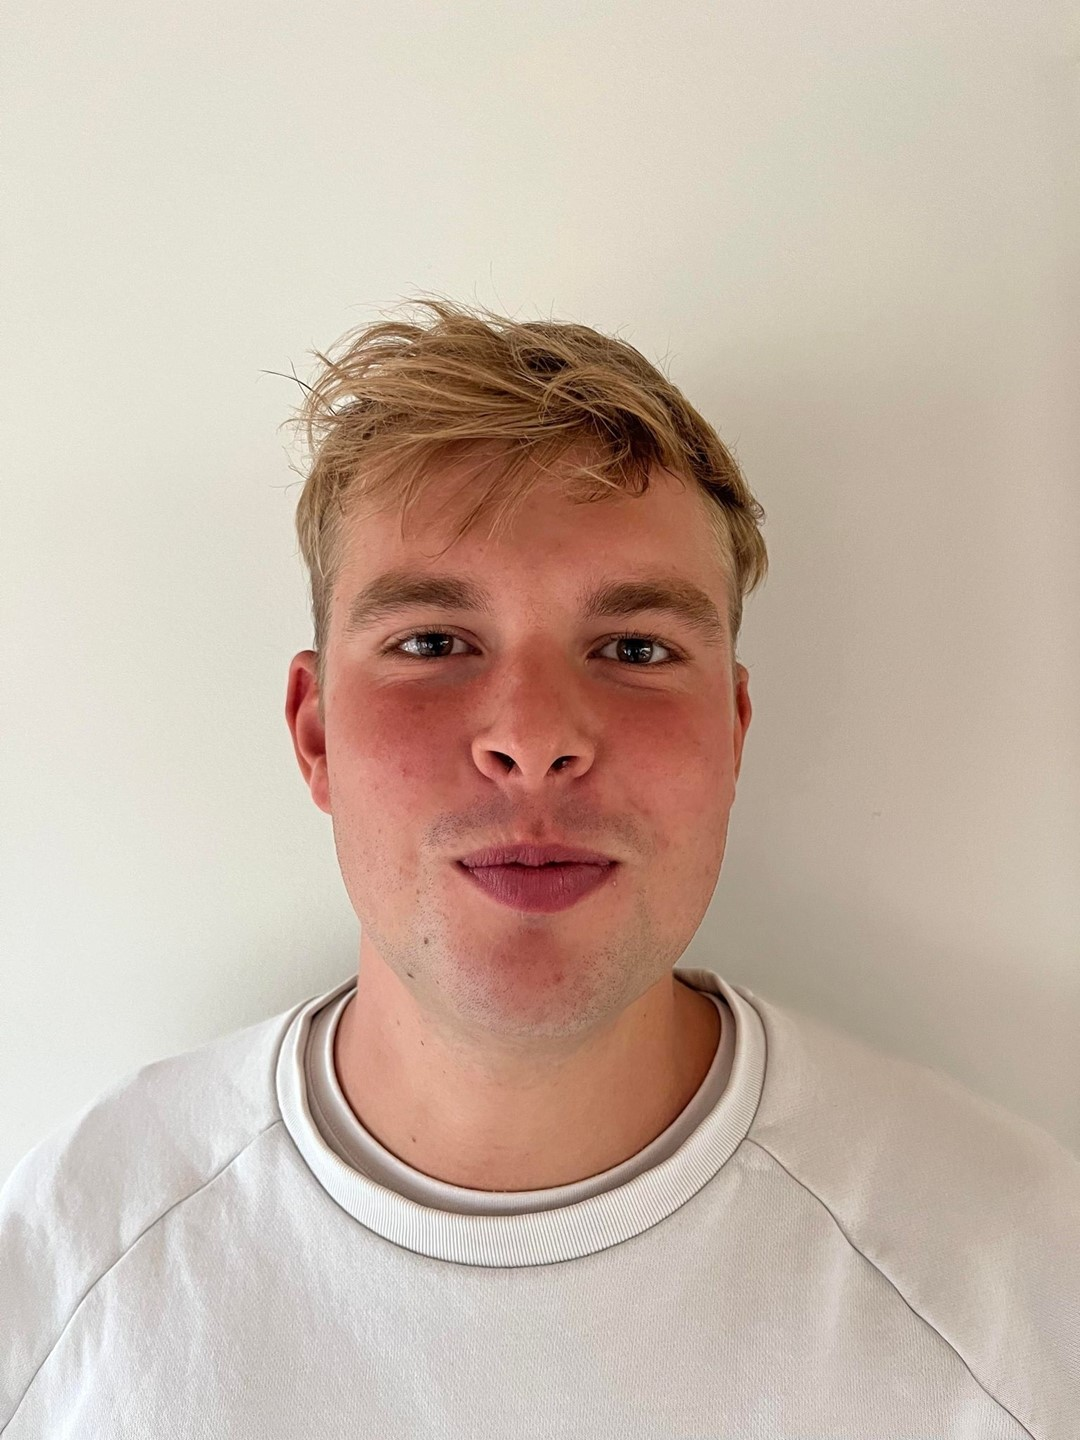
\includegraphics[width=0.2\textwidth]{Billeder/FotoMads.jpg} & 
\includegraphics[width=0.2\textwidth]{Billeder/EsbenFoto.png} & Esben Skovmand Elnegaard \vfill s224555  \\
    Jarl Boyd Roest\vfill s224556 & 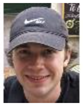
\includegraphics[width=0.2\textwidth]{Billeder/JarlFoto.png}
    \end{tabular}

    \vfill
    
    
    \vspace{1cm}
    \LARGE
    18. september 2022

    \vspace{1cm}
    
\end{center}
\end{titlepage}


\normalsize
\begin{abstract}
     Denne rapport indeholder et terningespil, som er blevet udviklet på baggrund af en række krav fra kunden. Under arbejdet med terningespillet har vi hele tiden teste programmet og lavet overvejelser over om det opfylder kravene fra kunden. Derudover har vi lavet analyserede kravene ved at lave en Use Case.  Til det har vi brugt den iterativ metode. Under processen har vi testet de 2 terninger som skal indgå i terningespillet, for at se om de er normaltfordelt rigtigt. Afslutningsvis er der blevet konkluderet at at vi har opfyldt kravene fra kunden og de er blevet implementerede i Intellij.     
\end{abstract}
\break

\tableofcontents

\break

\section{Timeregnskab}
\begin{itemize}
\item
Arbejdsdag 1 (19-09-2022): 2,5 timer
\item
Arbejdsdag 2 (21-09-2022): 3 timer
\item
Arbejdsdag 3 (23-09-2022): 2 timer
\item
Arbejdsdag 4 (26-09-2022): 2,5 timer
\item
Arbejdsdag 5 (27-09-2022): 2 timer
\item
Arbejdsdag 6 (28-09-2022): 2,5 time
\item
Arbejdsdag 7 (30-09-2022): 3 timer
\end{itemize}

\section{Indledning}

Denne rapport dokumenterer udviklingen af spillet Terningespil, der er udviklet på baggrund af kundens vision, kundens krav, samt vejledningen af projektlederen. Vi har forsøgt at følge (R)UP - metoden ved at være risikodrevet og fleksible i udviklingsprocessen. Vi har løbende opdateret vores opgaveprioritering og sat nye mål for de næste arbejdsdage. Vi har lavet forskellige artifakter til at hjælpe os i at forme det produkt der opfylder kundens krav mest. 


\section{Projekt-planlægning}
\begin {itemize}
\item [\textbf{Begyndelsen:}]Vi strukturerede, umiddelbart efter feedback fra projektlederen, en plan for udviklingen af projektet og programmet jf. kravspecifikationerne. Vi så på opgaverne og kravene til spillet, der var var slået på plads dag 1, og prioriterede opgaverne som følgende
 \item [\textbf{Uge 1:}]
 Opgaver prioriteret. (19-09-2022) udkast.
Versionsstyringen af programmet samt dokumentation for alle gruppemedlemmer
Use case(s), evt. diagrammer
Random nr generator samt test + terningkast og test.
Interface relaterede funktioner (navn, pointtæller, turskift, antal ture)
\item [\textbf{Uge 2:}]
Opdaterede opgaver (26-09-2022)
Opgaver løst:
Versionering af programmet
Diagram (sekvens)
test af terninger
interface kode: navn, pointtæller, turskift, antal ture
\item [\textbf{Nye opgaver:}]
Prioriteret:
Færdigudiviklen koden uden redepmtionfaktor
Opdatering af sekvens diagram samt klassediagram
Rapportere udvikling i rapporten.
Sekundære funktioner skal implementeres (coinflip)
\item []Dag 27-09-2022]
\item [\textbf{Opgaver løst:}] Alt kode til terningekastspillet inkl. redeptiomfaktor.
\item [Nye opgaver]:Prioriteret: Opdatering og commit af sekvens- samt domæne diagram. Fully dressed Use-case beskrivelse af main use case + alt flow (redemption). Implementering af GUI.
\item [Dag 28-09-2022]
\item Opgaver færdige:
\item Fejl i redemption loop fikset. Introduktion, dokumentering af test-af-terninger, design-klassediagram, samt use-case-beskrivelse færdiggjort.

\item [Nye opgaver]
\item Sidste opdatering af sekvensdiagram og færdiggørelse af rapport
\item 
\end {itemize}

 
\section{Krav/Analyse}
For at kunne lave en mere præcis kravsspecifikation startede vi med at spørge vores projektleder om følgende spørgsmål:
\begin{itemize}
    \item [Q:] hvilken version af Java har maskinerne installeret?
            \subitem A: Den nyeste version (18).
    \item [Q:]Hvilke input-metoder er tilgængelig?
            \subitem A: Både mus og tastatur.
    \item [Q:]Skal de 2 spillere have samme input-metode?
            \subitem A: De skal ikke, men kan godt.
    \item [Q:]Skal pointene være synlige for alle spillere eller blot nogle?
            \subitem A: Ja, synlige for alle.
    \item [Q:]Kan spillerne ende med mere end 40 point?
            \subitem A: Ja
    \item [Q:]Er vinderen den der når 40 point først? Hvad hvis de rammer 40 point på samme tur?
            \subitem A: Det er antallet af ture der tæller. Hvis begge spillere får 40 eller over, i samme tur, er vinderen den der slår højest i næste slag. Hvis lige fortsættes dette.
    \item [Q:]Hvad er et almindeligt menneske?
            \subitem A: Alle der besidder over 8. klasse pc færdighed, er op til 80 år gamle og har et almindeligt helbred.
    \item [Q:] Skal spillerne have navne?
            \subitem A: Ja
    \item [Q:]Hvem skal starte?
            \subitem A: Dette bestemmes ved et "coin flip". Altså helt tilfældigt.
    \item [Q:]Hvad er formålet med testen. Hvad ønskes der testet udover systemet funktionalitet som helhed?
        \subitem A: At de virtuelle terninger, statistisk opfører sig som normale terninger.
\end{itemize}

\noindent Baseret på dette har vi produceret en fully dressed use case beskrivelse for use casen: "Spil terningespil"

\subsection{Use case beskrivelse}
\textbf{Scope:} Spil terningespil\\
\textbf{Level:} Spillere\\
\textbf{Primary actor:} Spiller 1 og spiller 2\\
\textbf{Stakeholders and interests:}\\
-Spillere: Vil have et underholdene spil der virker hurtigt og korrekt.\\
-Projektlederne: Vil gerne kunne tilfredsstille kundens ønsker.\\
-kunden: Vil gerne have et spil, der kan spilles på DTU's databarer.\\
\textbf{Preconditions:} Der er styresystemet "Windows" på maskinerne og den nyeste version af Java.\\
\textbf{Succes Guarantee:} Spillet afsluttes og angiver en vinder.\\
\textbf{Main Succes Scenario:}\\
\begin{enumerate}
\itemsep-0.5em
    \item Spillerne indtaster deres navne en af gangen
    \item Systemet bestemmer vha. et coinflip hvilken af de to spillere der starter
    \item Vinderen af coinflippet slår med terningerne
    \item Systemet lægger øjnene på terningerne sammen, tæller dem som points og informere spilleren om dennes samlede point
    \item Den anden spiller slår nu med terningerne
    \item Systemet lægger øjnene på terningerne sammen, tæller dem som points og informere spilleren om dennes samlede point\\
    \textit{Punkterne 3-6 gentages indtil en af spillerne opnår 40 eller flere points}
    \item Systemet fortæller spillerne hvem der har vundet
\end{enumerate}

\textbf{Extensions:}
\begin{enumerate}
\itemsep-0.5em
    \item [7a.] Begge spillere opnår 40 point i samme runde
    \subitem 1. Systemet giver nu mulighed for at hver spiller kan kaste terningerne igen. Spilleren der slår  højest med dette ene kast vinder spillet.
    \subitem 2. Hvis de to spilleres slag har samme værdi starter de igen fra punkt 7a.1
\end{enumerate}
\textbf{Special Requirements:} Spillet vil kræve at spillerne kan skiftes til at benytte den samme input-metode\\
\textbf{Frequency of Occurence:} Spillet skal kunne gentages igen og igen\\
\textbf{Open Issues:} \\
-Skal spillerne have mulighed for at fortsætte et nyt spil med samme navne efter det første?\\



\section{Design}
For at finde frem til vores design startede vi med at med at lave et groft sekvensdiagram. så vi kunne få et overblik over rækkefølgen for klasser, objekter og metoder.\\
INDSÆT SEKVENSDIAGRAM (STARTEN) MÅSKE OGSÅ DESIGN-KLASSE-DIAGRAM\\

\begin{figure}[h]
    \centering
    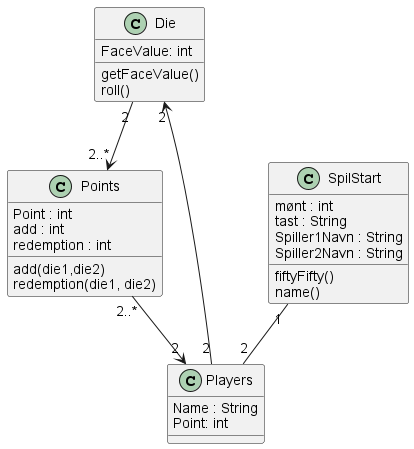
\includegraphics[width = 0.5\textwidth]{Billeder/ClassDiagram.png}
    \caption{Design-klassediagram}
    \label{fig:Design-klassediagram}
\end{figure}

Herefter var planen at starte med at implementere det funktionelle krav som enten bar mest risiko eller var vigtigst for spillet. Vi prioriterede derfor kravene således

\begin{enumerate}
\itemsep-0.4em
    \item Terninger - 2 stk. der kan kastes for at ændre deres øjenværdi
    \item Points - Tæller øjenværdierne fra de to terninger sammen
    \item Spillere - 2 stk. der hver har sine egne points og kan tildeles navne
    \item Afslutning - erklærer en vinder baseret på points og slutter spillet
    \item Redemption - Håndterer situation hvor begge spillere når 40 points eller over
\end{enumerate}


\section{Implementering}

\section{Test}
Der er blevet bedt om en test af de to terninger, som indgår i vores terningespil. Hensigten ved at teste terningerne er at se på sandsynligheden for de forskellige udfald. 
\footnote{https://emu.dk/sites/default/files/2020-06/normalfordelingen.pdf, side 7} De forskellige udfald skal stemmer overens med normalfordelingen for to terninger. En normal fordeling er karakteriserede ved at have en ”klokke”formede kurve. 

Der vil automatisk være kast, som er hyppigere end andre, da der er flere kombinationer som kan give det samme. Det vil for eksempel være tallene  6, 7 og 8, som vil være de mest hyppige kast. Tallene 6, 7 og 8 er de mest hyppige kast fordi der er flest forskellige kombinationer, der fremkommer af disse tal. 
Normal fordelingen for 2 terninger kan ses på figur \footnote{https://emu.dk/sites/default/files/2020-06/normalfordelingen.pdf, side 19} 2

\begin{figure} [h]
    \centering
    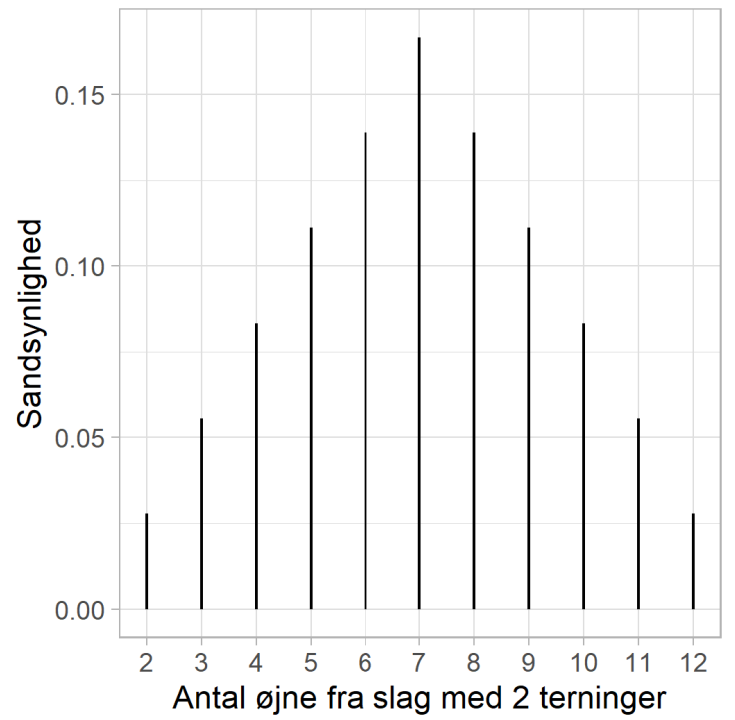
\includegraphics[width = 0.5\textwidth] {Billeder/normalfordelingen af 2 terninger.png}
    \caption{Sandsynlighed for at slå antal øjne}
    \label{fig:Sandsynligheden for at slå antal øjne}
\end{figure}


Vores test af terningerne er lavet i IntelliJ, som tager udgangspunkt i i de to terninger, som skal indgå i terningespillet. Terninger er blevet slået 10.000 gange for at få et mere præcis resultat. Man kan få et endnu mere præcis resultat, hvis man lavede flere terningkast, da det vil give flere observationer, og dermed en bedre normalfordeling. Derudover vil man få en pænere "klokke" formede kurve, hvis man havde et større interval af tal, da dette vil skabe en større spredning 
Testen af vores 2 terninger kan se i følgende figur 3

\begin{figure} [h]
    \centering
    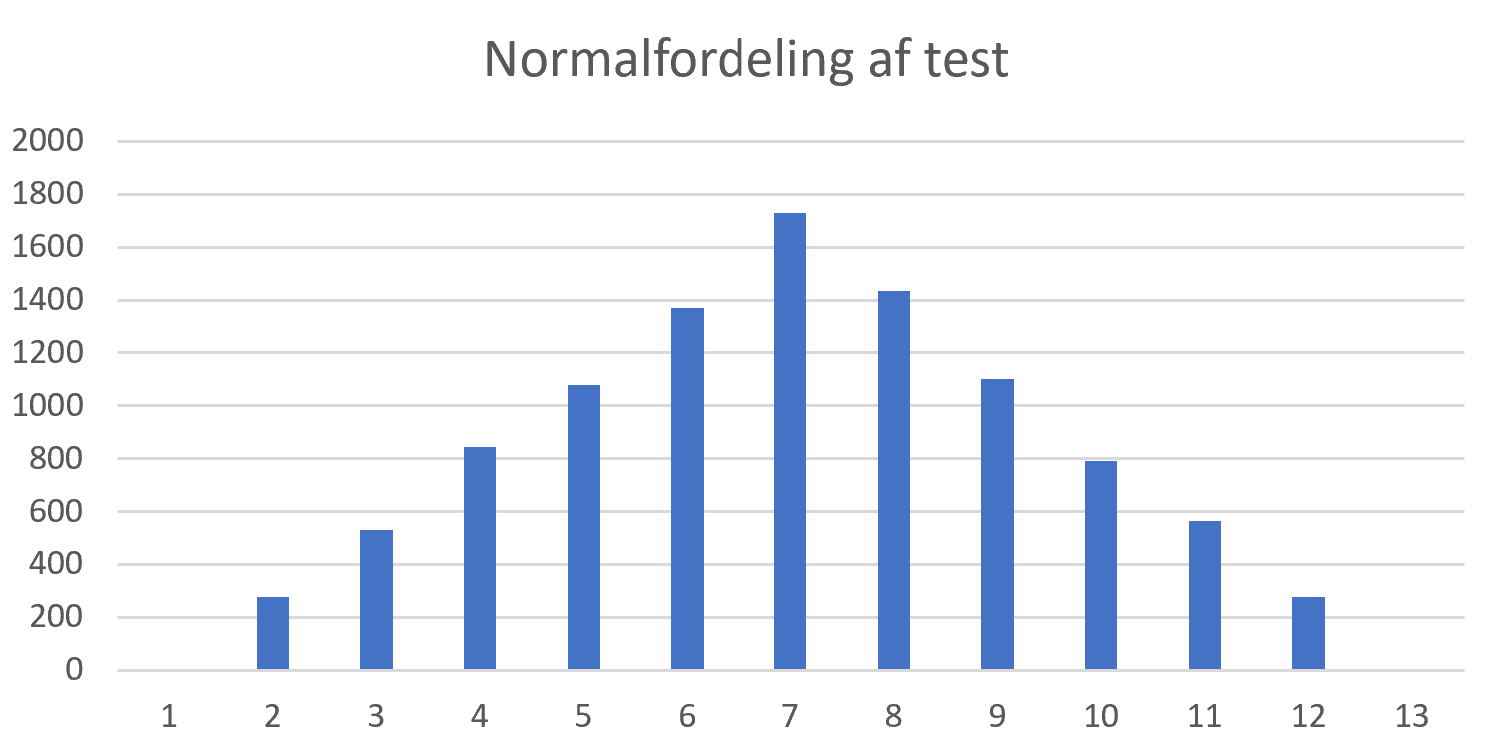
\includegraphics{Billeder/test af terninger.png}
    \caption {Normalfordelingen for terningekast med to terninger}
    \label{fig: Normalfordelingenm for terningekast}
\end{figure}
\item
\item
\item
\item
\item
\item
Ved at sammenligne figur 2 og 3, kan man hurtigt se, at de som udgangs er meget ens. Begge figurer har en det som man kan karakterisere som en "klokke" formede kurve, som også var målet. Der er nogle små ud svingninger i vores kurve, som gør at den ikke er helt præcis og dermed ikke ligner normalfordelinger af 2 terninger. Dette vil kunne løses sig ved at lave flere kast, der vil give flere observationer, som vil gøre det mere præcist. 


\section{Konklusion}
Vi har lavet et spil, der opfylder kundens krav. Dog er vi bevidste at vores kode kunne optimeres da meget af koden er genbrugt igennem programmet. Samtidig kunne vi have valgt at implementere koden i en GUI, men da det ikke var et krav og tiden var knap, udelod vi dette.
\item Læringsmål indtil videre:
Lav en test der faktisk kan teste hele spillet, så man ikke manuelt skal gennemgå hele spillet, hver gang man skal teste en ny linje kode.
\item Undgå at bruge for lang tid på at lave diagrammer og modeller. 


\section{Bilag}
\subsection{Litteratur}
\subsection{Kode}

\end{document}